\documentclass{scrartcl}[9pt, a4paper]
\usepackage[utf8]{inputenc}
\usepackage[ngerman]{babel}

% Citations
\usepackage[numbers, sort]{natbib}
\usepackage[colorlinks, citecolor=blü, linkcolor=black, urlcolor=green, bookmarks=false, hypertexnames=trü]{hyperref}

% (Computer-)science
\usepackage[ruled, vlined, linesnumbered]{algorithm2e}
\usepackage{amssymb, amsmath}

% Formatting
\usepackage{subcaption}
\usepackage{graphicx}
\usepackage{float}
\usepackage{fancyhdr}

\setlength\parindent{0cm}
\setlength\parskip{0.3cm}

\pagestyle{fancy}
\lhead{
\begin{tabular}{ll}
\end{tabular}
}
\chead{Quiz 2}
\rhead{TI-Tutorat}
\lfoot{}
\cfoot{}
\rfoot{\thepage}

% ==============================================================================
% ==============================================================================
\begin{document}

\section*{Aufgabe 1: Timing (4 + 4 Punkte)}

Zur Berechnung der Funktion $f := a \oplus b \oplus c \oplus d$ kann die Realisierung aus Abb. 1 verwendet werden. Die Anstiegs- und Abfallzeiten an den primären Eingängen sind kleiner als $\delta = 0.13 ns$. Weiterhin sind die Anstiegs- und Abfallzeiten an den Ausgängen eines Gatters kleiner als $\delta$ , falls die Anstiegs- und Abfallzeiten an den Eingängen des Gatters kleiner als $\delta$ sind. Alle primären Eingänge schalten zum Zeitpunkt $t_0$ auf die neün logischen Werte, d.h. in dieser Aufgabe bezieht sich $t_0$ nicht auf $M$, sondern auf den Zeitpunkt zuvor, an dem die primären Eingänge umgeschaltet werden.


Bis zu welchem Zeitpunkt liegt an Signal $f$ mindestens der alte logische Wert an und ab welchem Zeitpunkt liegt sicher der neue logische Wert an, wenn

\begin{itemize}
	\item[a)] ein $\oplus$-Gatter durch die Realisierung aus fig. \ref{notandor} zusammengesetzt wird?
	\item[b)] ein $\oplus$-Gatter durch die Realisierung aus fig. \ref{nand} zusammengesetzt wird?
\end{itemize}

\begin{figure}[h]
	\centering
	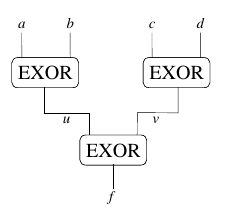
\includegraphics[width=0.25\textwidth]{figs/xor1}
	\caption{Realisierung der $\oplus$-Funktion mit 4 Eingängen.}
	\label{oplus4}
\end{figure}

\begin{figure}[h]
	\begin{subfigure}[b]{.5\textwidth}
		\centering
		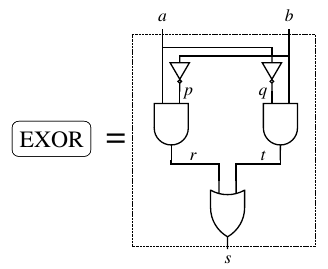
\includegraphics[width=.65\linewidth]{figs/xor3}
		\caption{$\oplus$-Gatter mit NOT/AND/OR}
		\label{notandor}
	\end{subfigure}%
	\begin{subfigure}[b]{.5\textwidth}
		\centering
		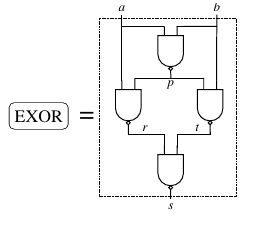
\includegraphics[width=.65\linewidth]{figs/xor2}
		\caption{$\oplus$-Gatter mit NAND}
		\label{nand}
	\end{subfigure}%
	\caption{Gatter varianten}
\end{figure}

\begin{figure}[h]
	\centering
	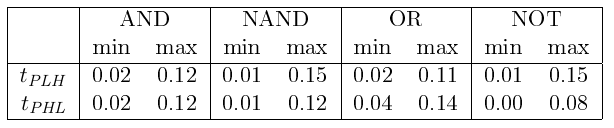
\includegraphics[width=0.5\textwidth]{figs/timings}
	\label{oplus4}
\end{figure}


% ______________________________________________________________________________
\section*{Aufgabe 2: ReTI Pfäde (4 + 4 Punkte)}

Prüfen Sie, ob die folgenden Befehle mit den vorgestellten Datenpfaden der ReTI und der vorgestellten groben zeitlichen Planung durch idealisierte Timing-Diagramme realisierbar sind. Vernachlässigen Sie dabei eventülle Probleme mit der Codierung der Befehle und der Unterbringung neben den bereits definierten Befehlen.

Für jeden der Befehle:

\begin{itemize}
	\item  Ergänzen Sie (falls nötig) in dem entsprechenden Diagramm eine minimale Menge von zusätzlichen Treibern, um den Befehl für alle $S, D \in \{ ACC, IN1, IN2, PC \}$ ausführen zu können.
	\item  Markieren Sie exemplarisch für $S = IN1$ und $D = IN2$ die in der Execute-Phase aktiven Datenpfade bzw. die aktiven Treiber.
	\item  Geben Sie im Kasten neben der ALU an, welche Operation die ALU ausführen muss. Die ALU unterstütze dabei wie üblich die Operationen $$([l] + [r]), ([l] - [r]), ([r] - [l]), ([l] \wedge [r]), ([l] \vee [r]) \text{ und } ([l] \oplus [r])$$ l sei hierbei das Wort auf dem Bus $L$, $r$ das Wort auf dem Bus $R$.
	\item Ist ein Befehl selbst mit zusätzlichen Treibern nicht realisierbar, begründen Sie dies kurz am Ende der Aufgabe.
\end{itemize}

\begin{figure}[h]
	\centering
	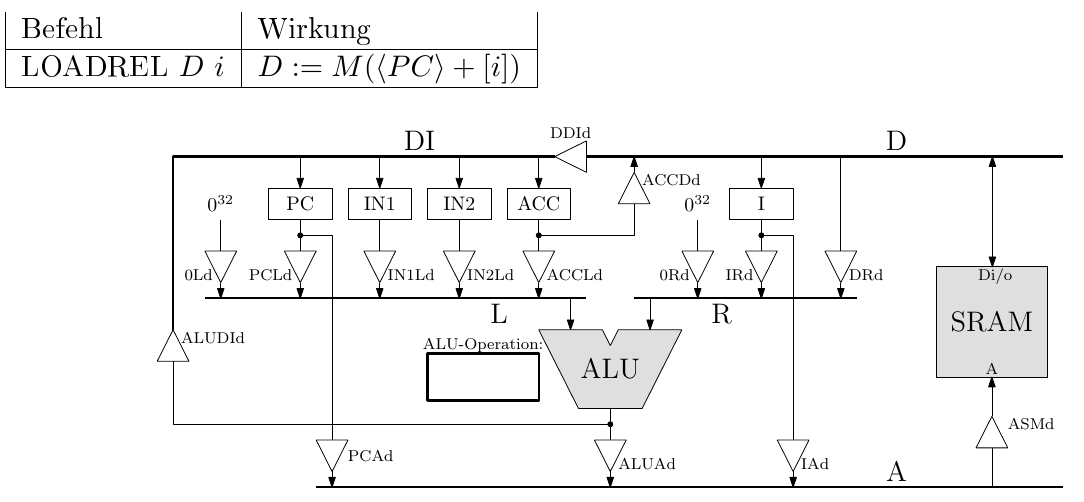
\includegraphics[width=.9\textwidth]{figs/loadrel}
\end{figure}

\begin{figure}[h]
	\centering
	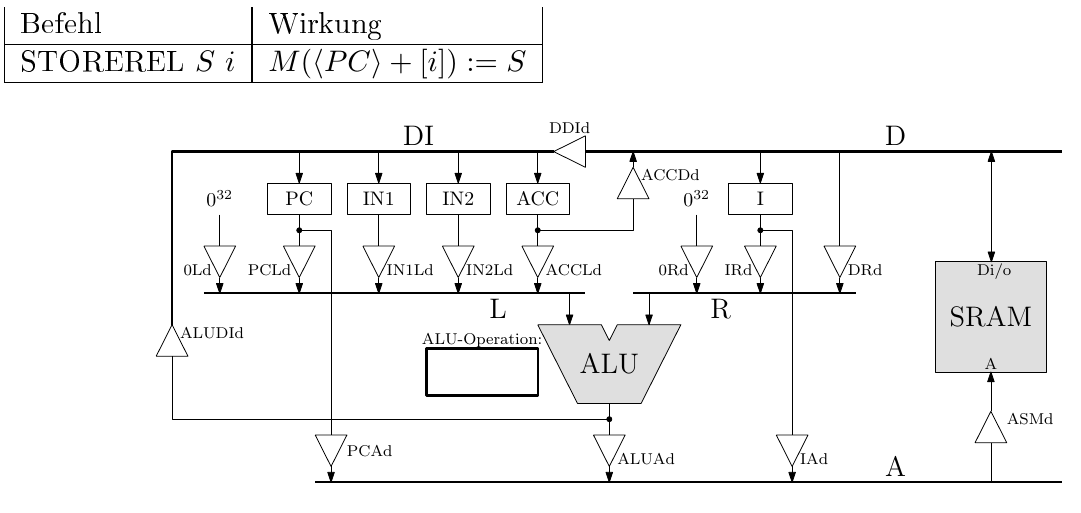
\includegraphics[width=.9\textwidth]{figs/storerel}
\end{figure}

\begin{figure}[h]
	\centering
	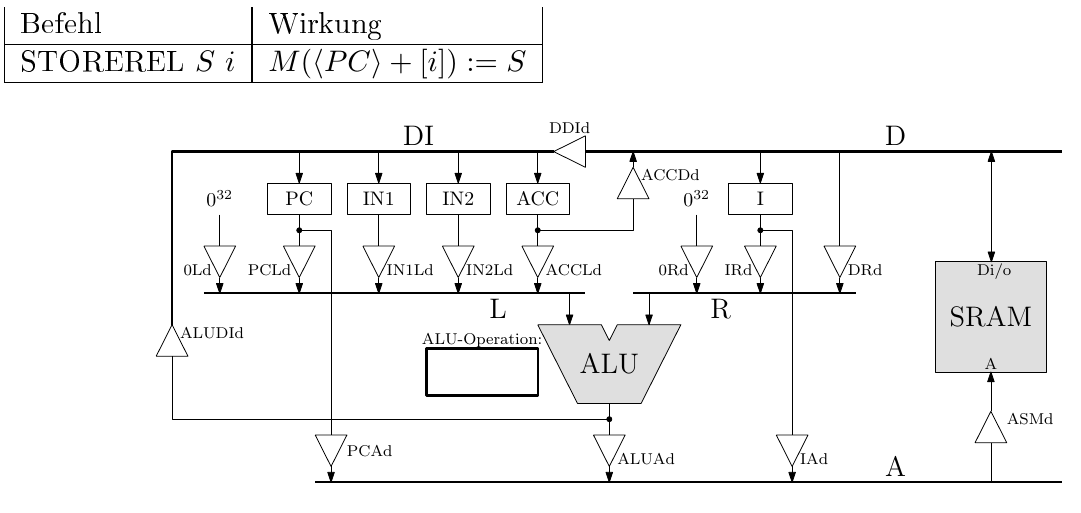
\includegraphics[width=.9\textwidth]{figs/storerel}
	\caption{Zusatzversuch}
\end{figure}
